\documentclass{article}
\usepackage{amsmath}
\usepackage{listings}

\usepackage{graphicx}
\graphicspath{ {./image/} }

\begin{document}

\section{CP2102}

\begin{enumerate}
    \item Connect the USB port to a desktop, a new serial port should be available.
    \item Using a serial tool(XCOM v2.0 in Windows or CuteCom in Ubuntu) to open the serial port, you will see some output. 
    \item Send "b", "y" or "r" to the device via the opened port, and the corresponding blue led, yellow led and red led will be toggled.
\end{enumerate}

\section{Speed Sensor}

\begin{enumerate}
    \item Connect external pulse signal generator to the speed sensor connectors.
    \item Open the serial port tool mentioned above, and you will read the frequencies of the pulse signal in the following format: "Speed: 0427 0427 0000 0499 0500 0499 0500 0427 0427 0854 0000 0000 0000 0499 0000 0000". Start with "Speed:", followed by 16 channels of frequency separated by a blank space. Each frequency contains 4 digits.   
    \item Note the input frequency range shall between 1~1k Hz, and will be round to an integer.
\end{enumerate}

\section{I2C Communication}
Two channels of i2c communication are used in the h750 board. One is for Communicating with PCA9685 and the other for BNO085. This test only scans the I2C addresses of those chips. 
\begin{enumerate}
    \item Open the serial port tool mentioned above. 
    \item You will see the output of the I2C addresses shown as Figure \ref{fig:i2c}
\end{enumerate}

\begin{figure}
    \centering
    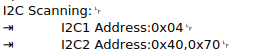
\includegraphics[totalheight=1.5cm]{i2c.png}
    \caption{I2C Message}
    \label{fig:i2c}
\end{figure}

The PCA9685 board has two I2C addresses(why?). The default I2C address of BNO085 is 0x4A.

\section{Brake}
4 channels of a timer are set to output PWM signals with the frequency of 1k Hz.
\begin{enumerate}
    \item Connect a voltage source(12V or 24V) to the connector of external high voltage. 
    \item The voltage on each channel shall be:
    \begin{enumerate}
        \item one third of the input voltage in Channel 1;
        \item two thirds of the input voltage in Channel 2;
        \item increasing from zero to the input voltage continuously in Channel 3, and
        \item decreasing from the input voltage to zero continuously in Channel 4
    \end{enumerate}    
 
\end{enumerate}

\section{ESC Signal Input}
Two input modes of ESC signal can be used.

\subsection{Manual(RC Transmitter) input switch}
\begin{itemize}
    \item Auto Mode: ESC and Servo pwm signals are calculated by the MPU.
    \item Manual Mode: ESC and Servo pwm signals are from an outside RC receiver.
\end{itemize} 
The input modes are switched by J?.
Test procedures:
\begin{enumerate}
    \item Open the serial port tool mentioned above. 
    \item Turn off the switch J?, the message via serial port shall contain the following strings: "Input Mode: Auto, Frequency: 50 Hz, ESC DutyCycle: 24\%, SERVO DutyCycle: 49\%". The esc output and servo output pins shall have the PWM signals output, whose frequency are 50 Hz both, and duty cycle 24 and 49, respectively.
    \item Turn on the swith J?, and connect the esc input pin and servo input pin to external PWM signals which should have the same frequency. The message should be like "Input Mode: Manual, Frequency: 63 Hz, ESC DutyCycle: 74\%, SERVO DutyCycle: 24\%", and The esc output and servo output pins shall have the same frequency and duty cycles as the input signals.
\end{enumerate}


The PWM signals from receiver are forward to STM32. In STM32 we use "PWM INPUT" functions of the timer to capture the frequence and the duty cycle of the pwm signals. Channel 1 of TIM5 is used to capture servo input and Channel 1 of TIM15 is used to capture ESC input. The output of servo and esc signals in STM32 are Channel 1 and Channel 2 of TIM3. Note output frequences would be the same as the two output channels are in the same timer. This is feasible since the frequences of the input signals are from the same receiver.
\begin{lstlisting}
	std_msgs::Float32MultiArray forces;
	forces.data = new std_msgs::Float32MultiArray::_data_type[8];
	forces.data_length = 8;
	//do not use the following:
	//forces.layout.dim = new std_msgs::MultiArrayDimension();

\end{lstlisting}
1. Select "PWM input on CH1", and set PSC to (X-1) where X is the frequence of APB1 Timer Clocks and APB2 Timer Clocks in MHz (Please set the two timer clocks the same to simplify settings). This leads the capture precision be 1/1M=1us. This is reasonable since the max value of the 16-bit ARR is 65535, the lowest frequence which can be detected is 1M/65535 = 15Hz. Typically the frequence of PWM signals for RC are 50Hz, the count is around 1M/50Hz = 20000. Note the TIM3 has a 32-bit ARR. 
Leave other settings default except check the global interrupt.

2. Insert the callback function:
\begin{lstlisting}

    void HAL_TIM_IC_CaptureCallback(TIM_HandleTypeDef *htim){

	if(htim->Instance==TIM5 && htim->Channel == HAL_TIM_ACTIVE_CHANNEL_1){
		uint32_t cl = HAL_TIM_ReadCapturedValue(htim, TIM_CHANNEL_1);
		uint32_t ch = HAL_TIM_ReadCapturedValue(htim, TIM_CHANNEL_2);


		freq1 = (float) TIMER_CLOCK_FREQ / (cl + 1);
		duty1 = (float) 100 * ch / cl;
		__HAL_TIM_SetCounter(htim,0);
		HAL_TIM_IC_Start_IT(&htim5, TIM_CHANNEL_1);
		HAL_TIM_IC_Start(&htim5, TIM_CHANNEL_2);
	}else if(htim->Instance==TIM15 && htim->Channel == HAL_TIM_ACTIVE_CHANNEL_1){
		uint32_t cl = HAL_TIM_ReadCapturedValue(htim, TIM_CHANNEL_1);
		uint32_t ch = HAL_TIM_ReadCapturedValue(htim, TIM_CHANNEL_2);
		__HAL_TIM_SetCounter(htim,0);
		freq2 = (float) TIMER_CLOCK_FREQ / (cl + 1);
		duty2 = (float) 100 * ch / cl;
		HAL_TIM_IC_Start_IT(&htim15, TIM_CHANNEL_1);
		HAL_TIM_IC_Start(&htim15, TIM_CHANNEL_2);
	}
}
\end{lstlisting}


Of course you have to start the timer inside the setup function after the timers is initialized. TIMER\_CLOCK\_FREQ is the APB Timer Clock.

3. Forward the frequence and duty cycle to TIM3. Using the following formula to set the ARR of TIM3:

\begin{equation}
    ARR = \frac{TIMER\_CLOCK\_FREQ}{frequence*(PSC+1)}-1
\end{equation}
Then using
\begin{lstlisting}
    __HAL_TIM_SetAutoreload()
\end{lstlisting} to set ARR value of TIM3.
Note this value only has to be set once.
And the Counter values of Channel 1 and Channel 2 are set to ARR*duty1 and ARR*duty2 respectively. This can be done inside callback function HAL\_TIM\_IC\_CaptureCallback.


\end{document}